% !TeX program=lualatex
% !TeX TXS-program:bibliography=txs:///biber

% ========
% Preamble
% ========

% -----
% Class
% -----
\documentclass[%
  paper=a4,%
  11pt,%
  oneside,%
  DIV=10,%
  BCOR=0mm,%
  headinclude=true,%
  headings=optiontoheadtoc,%
  headsepline=true,%
  footinclude=false,%
  parskip=half,%
  listof=leveldown,%
  captions=tableheading,%
  toc=sectionentrywithdots,%
%  draft,%
]{scrartcl}


% -----------
% Page layout
% -----------
% Customise spacing between lines
\usepackage{setspace}
\onehalfspacing
\setlength{\parindent}{1.5em}

% Afterpage flushing of floats
\usepackage{afterpage}

% Headers and footers
\usepackage[automark]{scrlayer-scrpage}
\pagestyle{scrheadings}
\automark[subsection]{section}
\clearpairofpagestyles
\ihead{\headmark}
\ohead{\pagemark}
\ofoot[\pagemark]{}


% TOC
\usepackage{multicol}
\BeforeStartingTOC[toc]{\begin{multicols}{2}}
\AfterStartingTOC[toc]{\end{multicols}}
\setlength{\columnseprule}{.5pt}
\setlength\columnsep{30pt}
\setcounter{tocdepth}{2}

% Landscape
\usepackage{lscape}

% -------------
% Maths support
% -------------
% Load maths packages
%% Typical packages
\usepackage{%
  amsmath,%
  amsthm,%
  amssymb,%
  mathrsfs,%
  mathtools,%
  gensymb,%
  braket,%
  mleftright,%
  xfrac,%
  interval,%
  rotating,%
  tabstackengine,%
}

% Settings for packages
%% interval: change open fences to round brackets
\intervalconfig{soft open fences}

%% mleftright: redefine \left as \mleft and \right as \mright
\mleftright

%% amsmath: equation numbering by section
\numberwithin{equation}{section}

%% tabstackengine
\TABstackMath
\TABbinary


% ------------------
% Scientific support
% ------------------
% Chemistry
\usepackage[version=4]{mhchem}

% Scientific typesetting
\usepackage{siunitx}
\DeclareSIUnit{\atomicunits}{a.u.}

% Lists
\usepackage[inline]{enumitem}


% ----------
% Typography
% ----------
% Context-sensitive quotation marks
\usepackage[english=british]{csquotes}

% Micro-typography
\usepackage[%
  activate={true, nocompatibility},%
  final,%
  tracking=true,%
  factor=1100,%
]{microtype}

% Reduce spacing between sc characters
\SetTracking{encoding={*}, shape=sc}{40}

% Disable -- and --- ligatures for tt family
\DisableLigatures[-,>,']{encoding=*, family=tt*}

% -------------------
% Font configurations
% -------------------
% Font support
\usepackage[tuenc, no-math]{fontspec}
\defaultfontfeatures{%
%  Ligatures=TeX,%
%  Numbers=Lining,%
}

% Main font selection
\setmainfont{Alegreya}[%
  Renderer=OpenType,
  Ligatures=TeX
]
% Renderer=Basic is needed to disable -- ligatures for tt family
\setmonofont[Renderer=OpenType]{Ubuntu Mono}

% Maths font selection
\usepackage[%
  math-style=ISO,%
  bold-style=ISO,%
  warnings-off={mathtools-colon},%
]{unicode-math}
\setmathfont{STIX Two Math}

% Bold version
\setmathfont{STIX Two Math}[%
  version=bold,%
  FakeBold=3.3,%
]

% Stylistic set selection for script variant
\setmathfont{STIX Two Math}[%
  range={scr, bfscr},%
  StylisticSet=1,%
]

% New font family
\newfontfamily\alegreyalocal{Alegreya}[Renderer=OpenType]
\newfontfamily\alegreyasclocal{Alegreya SC}[Renderer=OpenType]

%% Scale maths script and scriptscript sizes for text size 8
%\DeclareMathSizes{8}{8}{5.5}{5}
%
%% Avoid font size substitution with xfrac
%\usepackage{anyfontsize}


% ----------------
% Language support
% ----------------
% polyglossia requires fontspec
\usepackage{polyglossia}
\setmainlanguage[variant=british]{english}

% Date and time format
\usepackage{datetime}
\newdateformat{monthyeardate}{%
  \monthname[\THEMONTH] \THEYEAR
}


% -------
% Colours
% -------
\usepackage[svgnames, x11names, luatex, rgb]{xcolor}

% Colour aliases
\colorlet{LinkColour}{DarkCyan!50!Black}
\colorlet{PartColour}{Blue4!70!Black}
\colorlet{SectionColour}{DodgerBlue4}
\colorlet{SubsectionColour}{DodgerBlue3}
\colorlet{SubsubsectionColour}{DodgerBlue2}
\colorlet{ParagraphColour}{DodgerBlue1!70!Black}
\colorlet{HeaderFooterColour}{DeepSkyBlue4!70!Black}


% --------
% Diagrams
% --------
% Graphics
\usepackage{graphicx}

% TikZ & PGFPlots
\usepackage{pgfplots}

% Set up tikzexternalize
\usetikzlibrary{external}
\tikzexternalize
\newif\iftikzex
\ifdefined\notikzex
  \tikzexfalse
\else
  \tikzextrue
\fi
\tikzexternaldisable

\pgfplotsset{compat=1.16}

\usetikzlibrary{%
  calc,%
  luamath,%
  math,%
  positioning,%
  decorations.pathreplacing,%
  arrows.meta,%
  3d,%
  backgrounds,%
  patterns,%
}

\usepgfplotslibrary{%
  groupplots,%
  patchplots,%
  colormaps,%
}

\pgfplotscreateplotcyclelist{coloronly}{%
  {red},%
  {blue},%
  {black!60!green},%
  {black!20!orange},%
  {green!30!brown},%
  {blue!40!red},%
  {black!60!blue},%
  {black!40!yellow},%
  {red!50!pink},%
  {green!70!blue},%
}

% Command for tikzexternalize/includegraphics
\makeatletter
\newcommand*{\useexternalfile}[4]{
  \iftikzex
    \tikzsetnextfilename{tikzoutput/#4-output}
    \scalebox{#1}{\input{\tikzexternal@filenameprefix#4.tikz.tex}}
  \else
    \includegraphics[scale=#1, trim=#2 0 #3 0]{\tikzexternal@filenameprefix tikzoutput/#4-output.pdf}
  \fi
}
\makeatother

% Plot conditionals
\usepackage{xifthen}

% Float positioning
\usepackage{placeins}

% ------
% Tables
% ------
\usepackage{%
  booktabs,%
  multirow,%
  tabularx,%
  makecell,%
  pbox,%
  bigdelim,%
  array,%
}
\usepackage[export]{adjustbox}

% --------
% Captions
% --------
% Bold pre-texts in captions
\usepackage[%
  format=plain,%
  font={small, stretch=1.1},%
  labelfont=bf,%
  skip=5pt,%
]{caption}

% Subcaption support
\usepackage[%
  labelfont=rm,%
  subrefformat=parens,%
]{subcaption}

\captionsetup[subfigure]{justification=centering}
\captionsetup[subtable]{justification=centering}


% ------------------------
% References & bookmarking
% ------------------------
% Footnotes
\usepackage[perpage]{footmisc}
\renewcommand{\thefootnote}{\alph{footnote}}

% Footnote kerning with punctuation
% Do not use with option multiple for footmisc since this package has a different way of handling multiple footnotes.
\usepackage{fnpct}

% Bibliography
\usepackage[%
  sorting=none,%
  style=science,%
  articletitle=true,%
  autopunct=true,%
  autocite=superscript,%
  doi=true,%
  dateabbrev=true,%
  url=true,%
  isbn=false,%
  backend=biber,%
]{biblatex}
%\addbibresource{bib/hx_magnetic_symmetry.bib}
\bibliography{references}

%% Allow breaks in DOI
\setcounter{biburlnumpenalty}{100}
\setcounter{biburllcpenalty}{9000}


%% biblatex: new cite command to combine \citeauthor and \autocite
\newcommand*{\authorcite}[1]{\citeauthor{#1}\autocite{#1}}

% Bookmarking
%% hyperref must be loaded last, but before glossaries.
\usepackage[%
  hyperfootnotes=false,%
  hypertexnames=false,%
  hidelinks,%
]{hyperref}
\hypersetup{%
  bookmarksnumbered=true,%
  colorlinks=true,%
  citecolor=LinkColour,%
  linkcolor=LinkColour,%
}

% Cross-referencing
% cleveref must be loaded after hyperref
\usepackage[noabbrev, capitalise]{cleveref}

% ---------------
% List of symbols
% ---------------
% Load the glossaries package (after hyperref)
\usepackage[%
  symbols,% create list of symbols
  abbreviations,% create list of abbreviations
  nomain,%
  nonumberlist,%
  nogroupskip,%
  nopostdot,%
  automake%
]{glossaries-extra}

% Set acronym style
\setabbreviationstyle{long-short}

% Display glossaries in columns
\usepackage{glossary-mcols}

\setlength{\glsdescwidth}{\hsize}
\newglossarystyle{listofsymbolsstyle}{%
  \glossarystyle{list}%
  \renewcommand*{\glossaryentryfield}[5]{%
    \item[\glsentryitem{##1}\glstarget{##1}{##2}]%
    \hspace{0.5cm}##3\glspostdescription\space ##5}%
}

% Compute the widest entry just for the current glossary
\renewcommand{\glossarypreamble}{%
  \setlength{\parskip}{3pt}%
}
\glssetwidest[1]{symb:elecwfdet}

% Create an "ignored" list of symbols that will not be printed out
\newglossary[glignoredl]{ignored}{glignored}{glignoredin}{Ignored Glossary}

% Hyphenated long forms
\glsaddkey
  {hyphenated}        % new key
  {\relax}            % default value if "hyphenated" isn't used in \newglossaryentry
  {\glsentryhyphx}    % analogous to \glsentrytext
  {\Glsentryhyphx}    % analogous to \Glsentrytext
  {\glshyphx}         % analogous to \glstext
  {\Glshyphx}         % analogous to \Glstext
  {\GLShyphx}         % analogous to \GLStext
\newcommand{\GENglspostlinkhook}{%
  \ifglsused{\glslabel}{}{ (\glsentryshort{\glslabel})}\glsunset \glslabel}
\makeatletter
\newcommand\metadef[1]{%
  \expandafter\newcommand\csname gls#1\endcsname{%
    \@ifstar{\csname sgls#1\endcsname}{\csname ngls#1\endcsname}%
  }
  \@namedef{sgls#1}##1{{\let\glspostlinkhook \GENglspostlinkhook\expandafter\csname gls#1x\endcsname*{##1}}}%
  \@namedef{ngls#1}##1{{\let\glspostlinkhook \GENglspostlinkhook\expandafter\csname gls#1x\endcsname{##1}}}%
  \expandafter\newcommand\csname Gls#1\endcsname{%
    \@ifstar{\csname sGls#1\endcsname}{\csname nGls#1\endcsname}%
  }
  \@namedef{sGls#1}##1{{\let\glspostlinkhook \GENglspostlinkhook\expandafter\csname Gls#1x\endcsname*{##1}}}%
  \@namedef{nGls#1}##1{{\let\glspostlinkhook \GENglspostlinkhook\expandafter\csname Gls#1x\endcsname{##1}}}%
  \expandafter\newcommand\csname GLS#1\endcsname{%
    \@ifstar{\csname sGLS#1\endcsname}{\csname nGLS#1\endcsname}%
  }
  \@namedef{sGLS#1}##1{{\let\glspostlinkhook \GENglspostlinkhook\expandafter\csname GLS#1x\endcsname*{##1}}}%
  \@namedef{nGLS#1}##1{{\let\glspostlinkhook \GENglspostlinkhook\expandafter\csname GLS#1x\endcsname{##1}}}%
}
\makeatother

\metadef{hyph}


\makeglossaries
%\loadglsentries{symbols/symbols}
\loadglsentries{symbols/acronyms}


% ---------------
% Design features
% ---------------
% Counter depth
\setcounter{secnumdepth}{\subsubsectionnumdepth}
% Heading styles
%% Remove all end-of-counter dots
\renewcommand*{\autodot}{}

%% Use alphabets for subsubsection
\renewcommand\thesubsection{\thesection.\alph{subsection}}
\renewcommand\thesubsubsection{\thesubsection.\roman{subsubsection}}

%% KOMA-Script markups: adjust fonts and colours
\addtokomafont{disposition}{\alegreyalocal}
\addtokomafont{part}{\alegreyasclocal\Huge\color{PartColour}}
\addtokomafont{partnumber}{\alegreyasclocal\color{PartColour}}
\addtokomafont{section}{\Large\color{SectionColour}}
\addtokomafont{subsection}{\color{SubsectionColour}}
\addtokomafont{subsubsection}{\color{SubsubsectionColour}}
\addtokomafont{paragraph}{\itshape\color{ParagraphColour}}
\addtokomafont{subparagraph}{\bfseries}

%% KOMA_Script headers and footers: adjust fonts and colours
\addtokomafont{pageheadfoot}{\alegreyalocal\color{HeaderFooterColour}}
\addtokomafont{headsepline}{\color{HeaderFooterColour}}
\addtokomafont{pagenumber}{\alegreyalocal\color{HeaderFooterColour}}



%% Put section numbers in the margin
\renewcommand*{\sectionformat}{%
  \llap{\thesection\autodot\enskip}%
}

%% Put subsection numbers in the margin
\renewcommand*{\subsectionformat}{%
  \llap{\thesubsection\autodot\enskip}%
}

%% Put subsubsection numbers in the margin
\renewcommand*{\subsubsectionformat}{%
  \llap{\thesubsubsection\autodot\enskip}%
}


%% Adjust spacing around headings
\RedeclareSectionCommand[%
  afterskip=.25\baselineskip,%
]{section}
\RedeclareSectionCommand[%
  beforeskip=-.1\baselineskip,%
  afterskip=.1\baselineskip,%
]{subsection}
\RedeclareSectionCommand[%
  beforeskip=-.1\baselineskip,%
  afterskip=.1\baselineskip,%
]{subsubsection}
\RedeclareSectionCommand[%
  beforeskip=-.1\baselineskip,%
  afterskip=.1\baselineskip,%
]{paragraph}


% ---------------
% Special symbols
% ---------------
% Operators
\DeclareMathOperator{\im}{im}
\DeclareMathOperator{\id}{id}
\DeclareMathOperator{\tr}{tr}
\DeclareMathOperator{\spn}{span}
\DeclareMathOperator{\Ln}{Ln}
\DeclareMathOperator{\diag}{diag}
\DeclareMathOperator{\Sym}{Sym}
\DeclareMathOperator{\Arg}{Arg}

% Commands
%% Differential operator
\newcommand*{\D}{\symup{d}}

%% Transpose
\newcommand*{\T}{\symsfup{T}}

%% Vector operator
\newcommand*{\vecop}[1]{\hat{\symbfit{#1}}}

%% Latin abbreviations
\usepackage{xspace}
\newcommand*{\eg}{\textit{e.g.}\@\xspace}
\newcommand*{\ie}{\textit{i.e.}\@\xspace}
\newcommand*{\ca}{\textit{ca.}\@\xspace}
\newcommand*{\cf}{\textit{cf.}\@\xspace}

\makeatletter
\newcommand*{\etc}{%
    \@ifnextchar{.}%
        {\textit{etc}}%
        {\textit{etc}.\@\xspace}%
}
\makeatother



% ------------------------------
% Code listings and other frames
% ------------------------------
% Frames and boxes
\usepackage[most]{tcolorbox}

\tcbuselibrary{%
  minted,%
  breakable
}

%\usepackage{upquote}

% Non-copyable texts in PDF
\usepackage{%
  accsupp,%
}

\newcommand*{\noncopy}[1]{
  \BeginAccSupp{method=escape, ActualText={}}
  #1
  \EndAccSupp{}
}

% Listings environments

%% Minted style
\usemintedstyle{default}

%% Non-copyable line numbers
\renewcommand{\theFancyVerbLine}{\tiny\ttfamily\noncopy{\arabic{FancyVerbLine}}}

%% Non-copyable shell prompts
\newcommand{\LineWithPrompt}{%
  \def\FancyVerbFormatLine##1{\textcolor{red}{\noncopy{\$}}##1}%
}

%% Shell command environment
\NewTCBListing[%
  auto counter,%
  number within=section,%
  Crefname={Command}{Commands},%
]{bashcmd}{ s O{} m }{%
%  breakable,%
  enhanced,%
  colback=Seashell,%
  colframe=Grey!30!black,%
  listing only,%
%  before skip balanced=0pt,%
  comment above* listing,%
  IfBooleanTF={#1}
    {}%
    {comment={\centering \textbf{Command~\thetcbcounter:} #3\nopagebreak}},%
  left=3pt,%
  right=27pt,%
  listing engine=minted,%
  minted language=bash,%
  minted options={%
    breaklines,%
    autogobble,%
    stripall,%
    formatcom=\LineWithPrompt,%
    breaksymbolleft=\textcolor{gray}{\ensuremath{\noncopy{\hookrightarrow}}},%
    breaksymbolright=\textcolor{gray}{\ensuremath{\noncopy{\hookleftarrow}}},%
  },%
  title={\noncopy{\texttt{bash} command}},%
  #2
}

%% Shell output environment
\NewTCBListing[%
  use counter from=bashcmd,%
  Crefname={Output}{Outputs},%
]{bashoutput}{ s O{} m }{%
  enhanced,%
  colback=PapayaWhip,%
  colframe=Grey!30!black,%
  listing only,%
%  before skip balanced=0pt,%
  comment above* listing,%
  IfBooleanTF={#1}
    {}%
    {comment={\centering \textbf{Output~\thetcbcounter:} #3\nopagebreak}},%
  left=3pt,%
  right=3pt,%
  listing engine=minted,%
  minted language=bash,%
  minted options={%
    breaklines,%
    autogobble,%
    stripall,%
    breaksymbolleft=\textcolor{gray}{\ensuremath{\noncopy{\hookrightarrow}}},%
    breaksymbolright=\textcolor{gray}{\ensuremath{\noncopy{\hookleftarrow}}},%
  },%
  title={\noncopy{\texttt{bash} output}},%
  #2
}

%% Slurm file environment
% \readslurmscript[<options>]{caption}{filepath}
\NewTCBInputListing[%
  use counter from=bashcmd,%
  Crefname={Script}{Scripts},%
]{\readslurmscript}{ O{} m v }{%
%  breakable,%
  enhanced,%
  colback=Cornsilk,%
  colframe=Grey!30!black,%
  listing only,%
%  before skip balanced=0pt,%
  comment above* listing,%
  comment={\centering \textbf{Script~\thetcbcounter:} #2\nopagebreak},%
  left=3pt,%
  right=3pt,%
  listing engine=minted,%
  minted language=slurm,%
  minted options={%
    breaklines,%
    autogobble,%
    stripall,%
    linenos,%
    numbersep=3mm,%
    breaksymbolleft=\textcolor{gray}{\ensuremath{\noncopy{\hookrightarrow}}},%
    breaksymbolright=\textcolor{gray}{\ensuremath{\noncopy{\hookleftarrow}}},%
  },
  listing file={#3},%
  title={\noncopy{\texttt{SLURM} submission script:}\texttt{#3}},%
  #1
}

%% Shell script environment
% \readbashscript[<options>]{caption}{filepath}
\NewTCBInputListing[%
  use counter from=bashcmd,%
  Crefname={Script}{Scripts},%
]{\readbashscript}{ O{} m m }{%
  breakable,%
  enhanced,%
  colback=Cornsilk,%
  colframe=Grey!30!black,%
  listing only,%
%  before skip balanced=0pt,%
  comment above* listing,%
  comment={\centering \textbf{Script~\thetcbcounter:} #2\nopagebreak},%
  left=3pt,%
  right=3pt,%
  listing engine=minted,%
  minted language=bash,%
  minted options={%
    breaklines,%
    autogobble,%
    stripall,%
    linenos,%
    numbersep=3mm,%
    breaksymbolleft=\textcolor{gray}{\ensuremath{\noncopy{\hookrightarrow}}},%
    breaksymbolright=\textcolor{gray}{\ensuremath{\noncopy{\hookleftarrow}}},%
  },
  listing file={#3},%
  title={\noncopy{\texttt{bash} script:}\texttt{#3}},%
  #1
}

%% Generic text file environment
% \readbashscript[<options>]{file type}{caption}{filepath}
\NewTCBInputListing[%
  use counter from=bashcmd,%
  Crefname={File}{Files},%
]{\readtextfile}{ O{} m m m }{%
  breakable,%
  enhanced,%
  colback=Cornsilk,%
  colframe=Grey!30!black,%
  listing only,%
%  before skip balanced=0pt,%
  comment above* listing,%
  comment={\centering \textbf{File~\thetcbcounter:} #3\nopagebreak},%
  left=3pt,%
  right=3pt,%
  listing engine=minted,%
  minted language=text,%
  minted options={%
    breaklines,%
    autogobble,%
    stripall,%
    linenos,%
    numbersep=3mm,%
    breaksymbolleft=\textcolor{gray}{\ensuremath{\noncopy{\hookrightarrow}}},%
    breaksymbolright=\textcolor{gray}{\ensuremath{\noncopy{\hookleftarrow}}},%
  },
  listing file={#4},%
  title={\noncopy{#2:}\texttt{#4}},%
  #1
}

%% Task environment
\DeclareTColorBox[%
  auto counter,%
  %number within=section,%
  Crefname={Task}{Tasks},%
]{task}{ O{} m }{%
  enhanced,%
%  breakable,%
  title={Task~\thetcbcounter: #2\nopagebreak},%
  colframe=Grey!10!black,%
  colback=LightGoldenrod1,%
  colbacktitle=DarkGoldenrod1,%
  fonttitle=\bfseries,%
  coltitle=black,%
  left=3pt,%
  right=6pt,%
  top=12pt,%
  attach boxed title to top left={%
    xshift=9mm,%
    yshift=-0.25mm-\tcboxedtitleheight/2,%
    yshifttext=2mm-\tcboxedtitleheight/2,%
  },%
  boxed title style={%
    boxrule=0.5mm,
    frame code={%
      \path[tcb fill frame] ([xshift=-4mm]frame.west)
-- (frame.north west) -- (frame.north east) -- ([xshift=4mm]frame.east)
-- (frame.south east) -- (frame.south west) -- cycle;%
    },%
    interior code={%
      \path[tcb fill interior] ([xshift=-2mm]interior.west)
-- (interior.north west) -- (interior.north east)
-- ([xshift=2mm]interior.east) -- (interior.south east) -- (interior.south west)
-- cycle;%
    }%
  },%
  #1
}

%% Input file environment
\NewTCBListing[%
  auto counter,%
  number within=section,%
  Crefname={File}{Files},%
]{inpfile}{ O{} m m}{%
  breakable,%
  enhanced,%
  colback=Seashell,%
  colframe=Grey!30!black,%
  listing only,%
%  before skip balanced=0pt,%
  comment above* listing,%
  comment={\centering \textbf{File~\thetcbcounter:} #2},%
  left=3pt,%
  right=3pt,%
  listing engine=minted,%
  minted language=bash,%
  minted options={%
    breaklines,%
    autogobble,%
    stripall,%
    breaksymbolleft=\textcolor{gray}{\ensuremath{\noncopy{\hookrightarrow}}},%
    breaksymbolright=\textcolor{gray}{\ensuremath{\noncopy{\hookleftarrow}}},%
  },%
  title={\noncopy{\texttt{#3} file}},%
  #1
}

% -----------
% KOMA-Script
% -----------
% scrhack to prevent KOMA's "\float@addtolists detected!"
\usepackage{scrhack}
% Recalculate page margin based on loaded font
\recalctypearea


%% Metadata %%%%%%%%%%%%%%%%%%%%%%%%%%%%%%%%
  \title{Molecular Dynamics Workshop}
  \author{Ross Amory}
  \makeatletter
    \let\mytitle\@title
    \let\myauthor\@author
  \makeatother


\begin{document}
    \bgroup
    \noindent
    \begin{table}[H]
        \centering
        \begin{tabular}{cc}
            \begin{subfigure}{0.45\textwidth}
\includegraphics[height = 1.5cm,left]{Graphics/UKRI_BBSR_Council-Logo_Horiz-CMYK.eps}\end{subfigure}&  
            \begin{subfigure}{0.45\textwidth}
\includegraphics[height = 1.5cm,right]{Graphics/UoN_gradient_logo_CMYK.eps}\end{subfigure}\\
        \end{tabular}
    \end{table}
    \egroup

  %% Title
 \vspace{-0.5cm}
  \noindent
  \bgroup
    \alegreyalocal
    \renewcommand\arraystretch{1.5}
      \begin{tabular*}{\linewidth}{>{\centering\arraybackslash}m{\linewidth}}
        \hline
        \textbf{\alegreyasclocal\Large \mytitle}\\[-4pt]
        \myauthor{}\\[-8pt]
        pcyra2@nottingham.ac.uk\\
        School of Chemistry, University of Nottingham\\[-8pt] 
        \today\\
        \hline
      \end{tabular*}
  \egroup
  \thispagestyle{plain}

  % TOC
  \tableofcontents


\section{How to obtain software}
    \paragraph{}
    Here we will go through the steps to install all required software for this workshop. It is presumed that you are working either within a standard Linux terminal or using \gls{acr:wsl2} from within Windows. If you are using any other set-up, you will have to find out how to install the required software separately.

\subsection{Anaconda}
    \paragraph{}
    Install python and anaconda using the following commands. You should do this within a \gls{acr:wsl2} terminal if you are not natively working within linux.
    \begin{bashcmd}[label=listing:ANACONDAINST]{Commands to install anaconda and python.}
    wget https://repo.anaconda.com/archive/Anaconda3-2023.03-1-Linux-x86_64.sh
    sh Anaconda3-2023.03-1-Linux-x86_64.sh
    # Accept the license agreement and use all defaults suggested.
    \end{bashcmd}
\subsection{AMBER}
    \paragraph{}
    Install AmberTools22 using anaconda as this is the simplest way and suitable for this tutorial. 
    \begin{bashcmd}[label=listing:AMBERINST]{Commands to install AmberTools22}
    conda create --name AmberTools22
        y   # proceed with creating the AmberTools22 conda environment
    conda activate AmberTools22
    conda install -c conda-forge ambertools=22 compilers
        y   # proceed with installing
    \end{bashcmd}
\subsection{Acpype}
    \paragraph{}
    Install acpype using anaconda. In theory, this will also install ambertools, however, I find that having a separate install for both is best as you have greater control when just using amber.
    \begin{bashcmd}[label=listing:ACPYPEINST]{Commands to install Acpype}
    conda create --name acpype
        y   # proceed with creating the environment
    conda activate acpype
    conda install -c conda-forge acpype
        y   # proceed with installing
    \end{bashcmd}


\subsection{gnina} 
    \paragraph{}
    Below is the quick way of installing gnina. It simply downloads a pre-compiled binary of the software for an individual to use, however it is strongly recommended that you download the source code and compile it yourself for a more optimised experience.
    \begin{bashcmd}[label=listing:gninaINST]{Commands to install gnina.}
    wget https://github.com/gnina/gnina/releases/download/v1.0.3/gnina
    chmod +x gnina    
    # It is then recommended to add this to your PATH, .bashrc or modules in order to easily run this later in the workshop.
    \end{bashcmd}
\section{Theory}
    \paragraph{}
    In this section, a brief introduction to the theory behind the activities performed in the workshop. This will not however be a comprehensive theory section however, and further reading is strongly recommended to understand the methods.

\subsection{Molecular Dynamics}
\paragraph{}
Due to the size of biological systems, current computational power is unable to simulate every atom within an enzyme at a true quantum mechanical (QM) level and so some approximations must be made in order to simplify the system. The traditional method for simulating large biological molecules such as enzymes is to use a classical physics (Molecular Mechanics MM) approach (Equation: \ref{eq:EMM}), which includes using empirical force fields derived from classical physics in order to describe the system. The use of classical physics allows much simpler calculations and so increases computational efficiency dramatically, allowing the simulation of millions of atoms in a relatively short time scale. 

\begin{equation}
\label{eq:EMM}
\begin{split}
E_{Total} & = E_{Bonded} + E_{Non-Bonded} \\
E_{Bonded} & = E_{Bond} + E_{Angle} + E_{Dihedral} \\
E_{Non-Bonded} & = E_{Electrostatic} + E_{van der Waals} \\
\end{split}
\end{equation}

\paragraph{}
Molecular mechanics requires empirical forcefields\cite{Ponder2003ForceSimulations} to describe the behaviours of different atoms (and more importantly biological residues) to describe the energies of the different interactions within a system and so selecting a suitable forcefield which has been parametrised for your use case is important for achieving accurate results. For enzymes, the two most commonly used forcefields are CHARMM\cite{Vanommeslaeghe2009CHARMMFields} and AMBER\cite{Maier2015Ff14SB:Ff99SB} which were both parametrised for proteins and nucleic acids. 

\paragraph{}
These MM methods can be combined with QM methods in order to calculate the reaction center with high accuracy QM theory whilst also including interactions with the wider environment, specifically the electrostatic, dispersion and structural effects, which can control the structure of the reaction site and the thermodynamics of the system. In QM/MM you split the system into two or three sections (usually three) with your reaction site and any atoms which are known to be directly involved being put into the QM region. Then a thin layer around this region is included  as a hybrid zone which allows for communication between the two methods and used when the zone boundary intersects a covalent chemical bond. These atoms are usually calculated at both levels of theory. Finally the rest of the system is treated at the simplest level of theory (MM) (Figure: \ref{fig:Env}).

\subsection{Docking}

\subsection{GB/PBSA}\label{subsection:pbsa-theory}
\section{Workshop outline}
\label{sec:intro}
\tikzsetexternalprefix{./introduction/tikz/}

\subsection{Goals}
    \paragraph{}
    The main goal of this workshop is to give you a brief overview of what a standard \gls{acr:md} workflow would look like. We shall be covering some of the core techniques used to set-up and run a variety of different calculations including \textbf{molecular docking}, \textbf{molecular dynamics} and \textbf{free energy} calculations. We shall also briefly cover some analysis techniques available and some other resources available to further your understanding of the techniques used throughout. 

    \paragraph{}
    The steps of the workshop are as follows:
    \begin{itemize}
        \item Locate and download the crystal structure
        \item Dock the ligand into the active site
        \item Parameterise the ligand
        \item Create molecular dynamics input files
        \item Run a simple dynamics simulation
        \item Perform simple trajectory analysis
        \item Calculate the binding energy of the ligand
    \end{itemize}


\subsection{Software}
    \paragraph{}
    The key software that we will be using for this workshop all free to use and should be simple to access and use. Most of the software however requires a basic understanding of how to use the \gls{acr:cli}. It is possible to use all of the software from within windows, however it is recommended to use linux for the smoothest experience. 

    \paragraph{}
    The required software for this workshop is as follows:
\begin{itemize}
    \item \href{https://www.anaconda.com/download/}{anaconda}
    \item \href{https://learn.microsoft.com/en-us/windows/wsl/install}{WSL2} (windows only)
    \item \href{https://ambermd.org/GetAmber.php}{AMBER} \footnote{It is recommended that you install the full (paid) version of amber for production dynamics due to the GPU support, however for individual machines and the purpose of this workshop, the conda binary distribution is okay.}
    \item \href{https://www.ks.uiuc.edu/Development/Download/download.cgi?PackageName=VMD}{VMD}
    \item \href{https://github.com/gnina/gnina}{gnina}
    \item \href{https://pypi.org/project/acpype/}{acpype} \footnote{A web server version of acpype is available \href{https://www.bio2byte.be/acpype/submit/}{here} for users unable to install, however installing this is highly recommended where possible.}
\end{itemize}

    \paragraph{}
    Although not required for this workshop, some other software that is available to assist with the \gls{acr:md} workflow are as follows:

\begin{itemize}
    \item CHARMM (\gls{acr:md} package)
    \item gromacs (Open source \gls{acr:md} package)
    \item CGenFF (Forcefield parameterisation tool for the CHARMM forcefield)
    \item pyMol (\gls{acr:gui} for molecular visualisation and manipulation)
    \item AutoDock4 (Open source docking software)
    \item YASARA (\gls{acr:gui} for the whole \gls{acr:md} workflow)
    \item Alphafold (Open source A.I. homology modelling software)
\end{itemize}



\section{File types and jargon}
    There are many different files that are required to run a molecular dynamics simulation. Although many of the files can be used interchangeably, some file types contain extra information which can be useful in specific use cases. 

\subsection{File types}
    \subsubsection{Structure}
    \paragraph{}
        The first group of file types that are crucial, not only to molecular dynamics but to all of computational chemistry are coordinate or structure files. The most common version of these are \enquote{.xyz} files which contain the elemental information as well as the 3D spatial coordinates. A simple coordinate file must contain the 3D spatial coordinates of all particles in the system. There are many other pieces of information that can be entered into a structure file such as atomic elements, atom types, chemical charges and bonding information. Open Babel is a tool that has the ability to convert between many different structure file formats and can be incredibly useful when working with a variety of different structure files.

    \begin{table}[H]
        \centering
        \begin{tabular}{@{}cll@{}}
            \toprule
           \multicolumn{1}{l}{\textbf{Extension}}  &  \textbf{Extra Information} & \textbf{Human Readable} \\ \midrule
           .xyz & Elements, Number of atoms & Yes \\
           .pdb & Elements, Residue names, Atom types, Protein information  & Yes \\
           .mol2 & Atom types, Bonds, Charges, Molecule name & Yes \\
           .rst7 & Number of atoms, Periodic cell vectors & Yes \\
           .ncrst & Number of atoms, Velocities, Periodic cell vectors & No \\
           \bottomrule
        \end{tabular}
        \caption{A non-exhaustive list of structural file types that are used within the molecular dynamics workflow.}
        \label{tab:structFiles}
    \end{table}

    \subsubsection{Parameter files}
    \paragraph{}
        Although structure files often contain enough information in order to visualise or run simple calculations on the systems, when a large number of atoms or molecules are included in the system it is often sensible to split these into two files. This is where parameter files become useful as they contain a list of extra information about the particles in the system. This is also useful for dynamical systems where the parameters of the particles do not change but the positional information does. Parameter files are mainly used within molecular dynamics simulations for this reason and it is important to note that they can also be known as topology files within other simulation packages. The parameter file format that we will be using within the workshop is the \enquote{.parm7} file type from Amber.

    \subsubsection{Trajectory files}
    \paragraph{}
        Trajectory files in their simplest form are a combination of structure files that allow you to follow the movement of particles within a simulation. As they can contain many different sets of coordinates for a single system, these files can often become large and so they usually contain only the spatial information of the system and so require a parameter file to be understood. There are two types of trajectory files that we will see throughout the workshop; \enquote{.nc} and \enquote{.binpos}. Both of these files are in binary format in order to reduce the file size and the main reason for using \enquote{.binpos} files are that \enquote{.nc} files cannot be opened in the Windows version of \texttt{VMD}.

    \subsubsection{Input files}
    \paragraph{}
        Due to the functionality of most scientific software, it is often useful to create input files that tell the software what type of calculation you are planning to undertake. These are usually plain text files that have specific keywords that are understood by the software. 

    \subsubsection{Data files}
    \paragraph{}
        When running molecular dynamics, you can quickly become overwhelmed by the ammount of data that can be outputted. It is therefore often useful to extract specific data into \enquote{.dat} files which are usually tabular files that contain plottable data for a specific property. The \enquote{.dat} file extension is not exclusive to this usage however and not all of these can be quickly plotted so it is often useful to check what data is contained within such files. 
\section{Tasks}
\label{sec:Tasks}
\subsection{Initial Tasks}
    \begin{task}[label=task:setup]{Set up the directory structure for the workshop.}
    Create directories for:
        \begin{enumerate}[label=(\alph*)]
            \item Structure files
            \item Docking simulations
            \item \gls{acr:md} simulations
            \item Simulation analysis
        \end{enumerate}
    \end{task}

    \paragraph{}
    Firstly, like whenever starting any new project, a working directory needs to be created. This can be done either using the \gls{acr:cli} in a terminal using the \enquote{\texttt{mkdir}} command, or using a \gls{acr:gui} file manager. Commands to do this can be found in the cheat codes \cref{listing:task1}.

\begin{bashoutput}[label=listing:folders]{Folder structure as shown by the \texttt{tree} command.}
    MD_Workshop
    ├── Structures
    ├── Docking
    ├── Dynamics
    ├── Analysis
    └── Free_Energy
\end{bashoutput}
    
    \begin{task}[label=task:Structures]{Obtaining the structure files.}
    \begin{enumerate}[label=(\alph*)]
        \item Obtain the protein crystal structure
        \begin{enumerate}[label=(\roman*)]
            \item Visit the protein database website
            \item Find the protein using code 1AZX
            \item Download the crystal structure
        \end{enumerate}
        \item Save the ligand coordinate files located in the workshop files.
    \end{enumerate}
  \end{task}

  \paragraph{}
  There are a few places where you can find and store crystal structure coordinates, however the main two that are used are \href{https://www.rcsb.org/}{rscb} and \href{https://www.uniprot.org/}{uniprot}. These websites are powerful tools, and often group multiple versions of the same protein. Most proteins are published on the rscb database however for unresolved crystal structures, uniprot sometimes also contains the alphafold\cite{} homology model structure. 

  \paragraph{}
  Although we will not be covering the theory or methods of homology modelling in this workshop, being aware of the technique could potentially be useful when working with an un-resolved protein. The method allows for an approximate structure to be generated using similar proteins as templates. A homology modelling program with growing popularity is the \href{https://www.deepmind.com/research/highlighted-research/alphafold}{alphafold}\cite{} program which uses artificial intelligence to estimate a crystal structure from a FASTA sequence.

  \paragraph{}
  To start this workshop, you will need to visit the rscb website and download the \enquote{pdb} file for the antithrombin/pentasaccharide protien complex which can be found using the code 1AZX.  If you google the protein code, it usually comes up as one of the first options also. If you have any problems with this then use the commands found in the cheat codes \cref{listing:task2}.
\subsection{Docking}
    \begin{task}[label=task:Docking]{Docking a ligand into the protein.}
        \begin{enumerate}[label=(\alph*)]
            \item Dock the ligand
            \item Check docked poses
        \end{enumerate}
    \end{task}

    \paragraph{}
        To run a \gls{acr:md} simulation of a ligand-protein complex, you first need a good start structure for the ligand docked into the protein. Luckily many protein structures are obtained with a ligand already docked into the active site and so these positions can be used as a starting point for docking our ligands. We shall be using gnina as it can take the \enquote{2BN.pdb} structure generated previously as an initial guess for the active site location.

    \begin{bashcmd}[label=cmd:gnina]{Basic input for gnina without GPU acceloration}
        gnina -r 1n23_monomer_NoLig.pdb -l LIG.mol2 --autobox_ligand 2BN.pdb  -o docked.mol2 --no_gpu 
    \end{bashcmd}

    \begin{table}[H]
    \centering
    \begin{tabular}{@{}cll@{}}
    \toprule
    \multicolumn{1}{l}{\textbf{Option}} & \textbf{Value}    & \textbf{Type} \\ \midrule
    \textendash r                                           & Receptor/Protein pdb file                 & Input     \\
    \textendash l                                           & Ligand file to be docked                  & Input     \\
    \textendash \textendash autobox\textunderscore ligand   & Stripped receptor/protein parameter file  & Input     \\
    \textendash o                                           & Output PDB file for docked poses          & Output    \\
    \textendash \textendash no\textunderscore gpu           & Switches off GPU acceleration             & Variable  \\
                                                            & (Not necessary if compiled correctly)    &           \\
    \bottomrule
    \end{tabular}
    \label{Tab:gninaVar}
    \caption{The input variables for gnina}
    \end{table}

    \paragraph{}
    The docked poses of the ligand can then be viewed using \texttt{VMD}, like when viewing the original complexed structure. You will however need to load in two files rather than one. It is easiest if you load your \enquote{1n23\textunderscore monomer\textunderscore NoLig.pdb} file first, then open the \enquote{docked.mol2} file once \texttt{VMD} has loaded (Figures \ref{fig:NewMol} and \ref{fig:LoadMol}). This will set the docked structures as \enquote{on top} meaning you can cycle through the different docked \enquote{Frames}. You should set your representation for your protein as \enquote{New Cartoon} (Figure \ref{fig:protRep}) and the representation for your docked ligand as \enquote{CPK} (Figure \ref{fig:dockRep}). 
        
    \begin{figure}[H]
        \centering
        \begin{minipage}{0.45\textwidth}
            \centering
            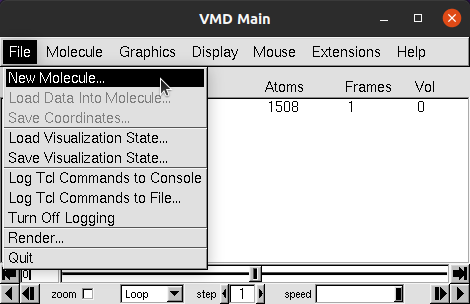
\includegraphics[width=0.9\textwidth]{Graphics/ScreenShots/NewMol.png}
            \captionof{figure}{How to load a new \\ molecule in VMD.}
            \label{fig:NewMol}
        \end{minipage}%
        \begin{minipage}{0.45\textwidth}
            \centering
            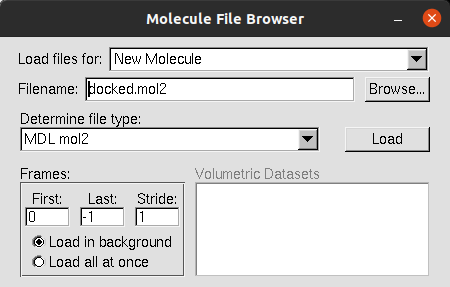
\includegraphics[width=0.9\textwidth]{Graphics/ScreenShots/docked_file.png}
            \captionof{figure}{How to select the file.}
            \label{fig:LoadMol}
        \end{minipage}
    \end{figure}

    \begin{figure}[H]
        \centering
        \begin{minipage}{0.45\textwidth}
            \centering
            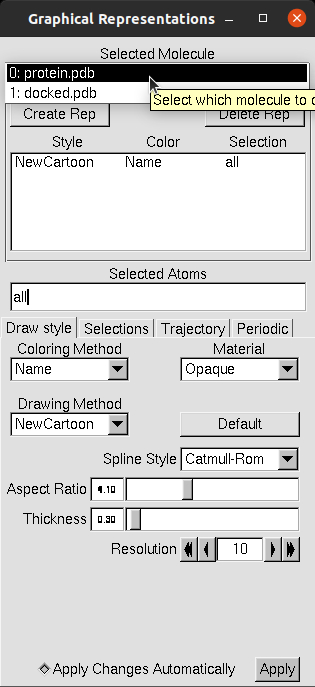
\includegraphics[height=0.5\textheight]{Graphics/ScreenShots/protein.png}
            \captionof{figure}{The representation for the protein.}
            \label{fig:protRep}
        \end{minipage}%
        \begin{minipage}{0.45\textwidth}
            \centering
            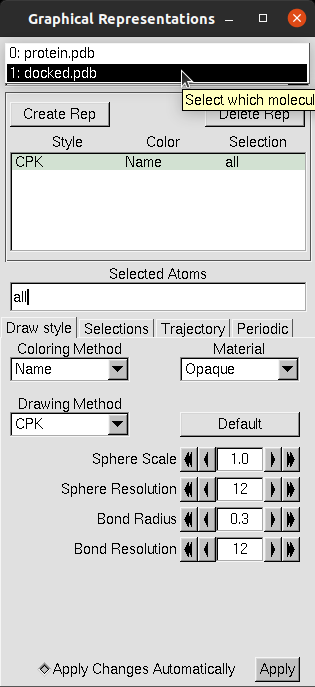
\includegraphics[height=0.5\textheight]{Graphics/ScreenShots/docked.png}
            \captionof{figure}{The representation for the \\ docked ligand.}
            \label{fig:dockRep}
        \end{minipage}
    \end{figure}

    \paragraph{}
        Finally, to use the docked pose for the molecular dynamics simulation you must extract the initial pose from the output coordinate file. You can either do this through the \gls{acr:gui} in VMD, or through the \gls{acr:cli}. It is recommended to use the \gls{acr:cli} as this is the fastest method and ensures that no structural manipulation takes place. To do this you copy the \enquote{docked.mol2} file to \enquote{pose\textunderscore 1.mol2}, then open in either vim or nano. From there you can simply delete the other docked poses from the file. (All the lines from the second \enquote{@<TRIPOS>MOLECULE}). The final docked file should look something similar to File \ref{out:mol2}.

    \begin{bashoutput}[label=out:mol2]{Docked pose output file.}
@<TRIPOS>MOLECULE
LIG.xyz
 10 9 0 0 0
SMALL
GASTEIGER

@<TRIPOS>ATOM
      1 C  42.7160   46.4533   46.0135 C.3     1  UNL1        0.0090
      2 C  43.7928   47.2054   46.6251 C.3     1  UNL1        0.0224
      3 C  43.7468   48.6707   46.5384 C.3     1  UNL1        0.0047
      4 C  44.7948   45.1707   47.5267 C.2     1  UNL1       -0.0049
      5 C  44.8573   46.4823   47.2270 C.2     1  UNL1       -0.0265
      6 C  41.4018   46.7840   46.8568 C.3     1  UNL1        0.0257
      7 C  41.7288   46.7347   48.3034 C.2     1  UNL1       -0.0346
      8 C  41.7967   45.6383   49.0677 C.2     1  UNL1       -0.0478
      9 C  42.1951   45.7469   50.5025 C.3     1  UNL1        0.0260
     10 C  41.5150   44.2497   48.5990 C.3     1  UNL1        0.0260
@<TRIPOS>BOND
     1     4     5    2
     2     5     2    1
     3     2     3    1
     4     2     1    1
     5     1     6    1
     6     6     7    1
     7     7     8    2
     8     8     9    1
     9     8    10    1
    \end{bashoutput}

    \paragraph{}
        You will notice that this docking procedure has removed the protons from our ligand so we shall have to manually add them back in. As our ligand is a carbocation, this process is more complicated than normal as automating the protonation of the molecule will also neutralise it. One way to fix this is to protonate the ligand to the neutral molecule, then manually remove the proton using a text editor. As \enquote{mol2} files contain bonding information, it is best to do this with a \enquote{.xyz} molecule file however.

    \begin{bashcmd}[label=cmd:addH]{Add hydrogen atoms and convert to .xyz.}
        obabel -imol2 pose_1.mol2 -oxyz -Opose_1.xyz -h   
        #This protonates and converts to xyz in one step.
    \end{bashcmd}

    \begin{bashoutput}[label=out:xyz]{Protonated neutral ligand.}
28
LIG.xyz
C         42.71600       46.45330       46.01350
C         43.79280       47.20540       46.62510
C         43.74680       48.67070       46.53840
C         44.79480       45.17070       47.52670
C         44.85730       46.48230       47.22700
C         41.40180       46.78400       46.85680
C         41.72880       46.73470       48.30340
C         41.79670       45.63830       49.06770
C         42.19510       45.74690       50.50250
C         41.51500       44.24970       48.59900
H         42.92737       45.40513       46.05305
H         42.59360       46.71744       44.98387
H         44.18007       47.67066       47.50740
H         43.32922       48.95932       45.59647
H         44.73798       49.06439       46.62478
H         43.13968       49.05599       47.33077
H         45.60368       44.70221       47.96403
H         43.93803       44.63420       47.31901
H         45.72789       46.99089       47.44709
H         40.64322       46.06240       46.63601
H         41.04477       47.75962       46.60067
H         41.92334       47.63624       48.76643
H         42.37555       46.77311       50.74586
H         43.08636       45.17877       50.66917
H         41.40891       45.36665       51.12073
H         41.23917       44.27121       47.56539
H         40.71320       43.83510       49.17356
H         42.39066       43.64721       48.72201
    
    \end{bashoutput}

    \paragraph{}
        When visualising the file, you will see that there is a proton on the carbocation. Selecting this atom shows us that it is atom index 12 and as \texttt{vmd} is \enquote{zero indexed}, it is the 13\textsuperscript{th} atom which needs removing. Delete this line in the \enquote{pose\textunderscore 1.xyz} file, and change the number at the top from 28 to 27 as this is the number of atoms in the molecule. Finally, we will convert back to \enquote{mol2} using obabel and \cref{cmd:xyzmol2}.

    \begin{bashcmd}[label=cmd:xyzmol2]{Convert back to mol2.}
        obabel -ixyz pose_1.xyz -omol2 -Opose_1.mol2
    \end{bashcmd}


    \paragraph{}
        Finally, you need to check that the hybridisation states for all of the carbons are correct. There should be 5 \enquote{C.2} carbons as there are 2 double bonds and 1 cationic carbon atom. It is likely that obabelen incorrectly identified the carbocation as \enquote{C.2} and so you should manually change this in your file (the carbocation should be carbon 2). The final file should look something like \cref{out:finaldocked} however we have excluded the bonding information for simplicity.

    \begin{bashoutput}[label=out:finaldocked]{The final structure for the docked molecule.}
@<TRIPOS>MOLECULE
LIG.xyz
 27 26 0 0 0
SMALL
GASTEIGER

@<TRIPOS>ATOM
    1 C  42.7160   46.4533   46.0135 C.3    1  UNL1    -0.0400
    2 C  43.7928   47.2054   46.6251 C.2    1  UNL1    -0.0052
    3 C  43.7468   48.6707   46.5384 C.3    1  UNL1    -0.0553
    4 C  44.7948   45.1707   47.5267 C.2    1  UNL1    -0.1021
    5 C  44.8573   46.4823   47.2270 C.2    1  UNL1    -0.0844
    6 C  41.4018   46.7840   46.8568 C.3    1  UNL1    -0.0337
    7 C  41.7288   46.7347   48.3034 C.2    1  UNL1    -0.0853
    8 C  41.7967   45.6383   49.0677 C.2    1  UNL1    -0.0796
    9 C  42.1951   45.7469   50.5025 C.3    1  UNL1    -0.0440
   10 C  41.5150   44.2497   48.5990 C.3    1  UNL1    -0.0440
   11 H  42.9274   45.4051   46.0530 H      1  UNL1     0.0277
   12 H  42.5936   46.7174   44.9839 H      1  UNL1     0.0277
   13 H  43.3292   48.9593   45.5965 H      1  UNL1     0.0238
   14 H  44.7380   49.0644   46.6248 H      1  UNL1     0.0238
   15 H  43.1397   49.0560   47.3308 H      1  UNL1     0.0238
   16 H  45.6037   44.7022   47.9640 H      1  UNL1     0.0532
   17 H  43.9380   44.6342   47.3190 H      1  UNL1     0.0532
   18 H  45.7279   46.9909   47.4471 H      1  UNL1     0.0572
   19 H  40.6432   46.0624   46.6360 H      1  UNL1     0.0308
   20 H  41.0448   47.7596   46.6007 H      1  UNL1     0.0308
   21 H  41.9233   47.6362   48.7664 H      1  UNL1     0.0571
   22 H  42.3755   46.7731   50.7459 H      1  UNL1     0.0274
   23 H  43.0864   45.1788   50.6692 H      1  UNL1     0.0274
   24 H  41.4089   45.3666   51.1207 H      1  UNL1     0.0274
   25 H  41.2392   44.2712   47.5654 H      1  UNL1     0.0274
   26 H  40.7132   43.8351   49.1736 H      1  UNL1     0.0274
   27 H  42.3907   43.6472   48.7220 H      1  UNL1     0.0274
@<TRIPOS>BOND
 # Bonding information
    \end{bashoutput}
\subsection{Molecular Dynamics Preparation}
\subsubsection{Parameterisation}
    \paragraph{}
        To run a molecular dynamics simulation, you first need to parameterise all of the atoms in the system. There are multiple different molecular dynamics force fields that contain standard parameters for common amino acids and some other small or simple molecules. For bigger or more complicated molecules however, you will need to create your own custom parameters. 

    \paragraph{}
        Although there is a rigorous method that can be undertaken to correctly parameterise complex ligands, including comparing the parameters with ab-initio calculations, we shall be using an automated method for speed and simplicity. \footnote{You can learn more about the rigorous process of parameterisation \href{http://ambermd.org/tutorials/basic/tutorial4b/}{here}.}

    \paragraph{}
        We shall be using the \texttt{acpype}\cite{} automated script to parameterise the ligands in this workshop, which combines the parameterisation tools offered by amber into a simple to use script. We shall be using \texttt{bcc} charges and the \texttt{gaff} atom typing so that it will be compatible with the \enquote{FF14SB} forcefield that we shall be using for the simulation.

    \begin{bashcmd}[label=listing:acpypeCMD]{How to use acpype.}
        conda activate acpype
        acpype -i LIG.pdb -c bcc -n NET_CHARGE -a gaff
    \end{bashcmd}
\subsection{Molecular Dynamics}

    \begin{task}[label=task:Dynamics]{Run a molecular dynamics simulation.}
        \begin{enumerate}[label=(\alph*)]
            \item Generate input files for:
            \begin{enumerate}[label=(\roman*)]
                \item Minimisation
                \item Heating
                \item Equilibration
                \item Production dynamics
            \end{enumerate}
            \item Run the simulations for:
            \begin{enumerate}[label=(\roman*)]
                \item Minimisation
                \item Heating
                \item Equilibration
                \item Production dynamics
            \end{enumerate}
        \end{enumerate}
    \end{task}


    \paragraph{}
        Once we have correctly generated our initial start coordinate system and the corresponding parameters, we can begin to run some dynamics simulations. A traditional dynamics simulation starts with a minimisation step which allows for any steric clashes or small structural problems within our initial system to be corrected before trying to introduce time. These steric clashes are very common as when you solvate the system, the water molecules are randomly placed and so can sometimes lead to problems if not fixed. It is common to run a multi-stage minimisation where you initially fix all atoms except for solvents and minimise, before slowly relaxing these restraints until a full system minimisation is performed. For the interest of time however we shall not be doing this.

\begin{inpfile}[label=file:minin]{Minimisation input file.}{sander}
initial minimisation script at 0k
&cntrl
  imin=1,       # initiate minimisation
  ntx=1,        # read coordinates with no velocities
  irest=0,      # don't restart the simulation
  maxcyc=10000, # 10000 minimisation steps
  ncyc=5000,    # 5000 steps of steepest gradient
  ntpr=10,      # print to mdout every 10 steps
  ntwx=0,       # don't print trajectory file
  cut=8.0,      # non-bonded cut off of 8 A
/

\end{inpfile}

    \paragraph{}
        Firstly we need to create an input file that tells amber what type of calculation we want to perform. These input files have many variables, however in alot of cases the default values are fine. We will first generate a simple minimisation input file called \enquote{min.in} that should look like \cref{file:minin} and should be saved to the \texttt{Dynamics} sub directory. The \enquote{start.rst7} and \enquote{complex.parm7} files generated from the previous step should also be copied here. Finally to run the initial minimisation, use \cref{cmd:minrun}.
        
\begin{bashcmd}[label=cmd:minrun]{Basic amber command to run the minimisation input file}
# If using the conda install or have no mpi compiled version:
sander -O -i min.in -o min.out -c start.rst7 -p complex.parm7 -inf min.mdinfo -r min.ncrst

# If compiled with mpi:
mpirun -np NUM_CORES sander.MPI -O -i min.in -o min.out -c start.rst7 -p complex.parm7 -inf min.mdinfo -r min.ncrst

# If using the full version of amber with GPU support:
pmemd.cuda -O -i min.in -o min.out -c start.rst7 -p complex.parm7 -inf min.mdinfo -r min.ncrst
### NOTE: Often the pmemd version struggles if large clashes are present. If you get an error, try switching to sander.
\end{bashcmd}

    \paragraph{}
        It should be noted that there are two main programs for running molecular dynamics within amber: \enquote{sander} and \enquote{pmemd}. If you are using the free version of amber (AmberTools), then you will only have access to  \enquote{sander}, however if you have the full version then you will also have \enquote{pmemd}. These two programs are functionally similar, with \texttt{pmemd} being an optimised and slimmed down code which can be run on GPU's where as \texttt{sander} is less optimised however much more rigorous. Both programs can be \texttt{mpi} accelerated however, so even with the free version of amber you can run some simple dynamics simulations. Some functionality of \texttt{sander} is lost when changing to \texttt{pmemd} however so always check to see if your calculation will work with your code.

    \begin{table}[H]
    \centering
    \begin{tabular}{@{}cll@{}}
    \toprule
    \multicolumn{1}{l}{\textbf{Option}} & \textbf{Value}    & \textbf{Type} \\ \midrule
    \textendash O                                           & Overwrite previous files                  & Variable  \\
    \textendash i                                           & Input file                                & Input     \\
    \textendash o                                           & Main output file                          & Output    \\
    \textendash c                                           & Simulation start coordinates              & Input     \\
    \textendash p                                           & Parameters for your system                & Input     \\
    \textendash inf                                         & Dynamics information about current step   & Output    \\
    \textendash r                                           & \enquote{Restart} file for the latest coordinates to be saved   &  Output          \\
    \textendash x                                           & \enquote{Trajectory} file for saving the coordinates every \enquote{ntwx} steps   &  Output        \\
    \bottomrule
    \end{tabular}
    \label{Tab:sanderVar}
    \caption{The input variables for sander or pmemd}
    \end{table}


    \paragraph{}
        Once minimisation is complete, the next step is to heat the system. Currently the temperature is at 0 k, however we need this to be at physiological temperature. This exact temperature can vary depending on what exactly you are simulating however for this workshop we shall heat to 300 k. The temperature of the system is determined by the average kinetic energy for all atoms and is related to temperature using the Maxwell-Boltzman distribution\cite{}. The temperature of the system is controlled by a thermostat which modifies the velocities of the atoms in order to keep the system at the desired temperature. 

    \paragraph{}
        To run the heating simulation, you first need to generate the input file and this should look similar to \cref{file:heatin}. You shall notice that we are now using more variables in the \texttt{\&cntrl} section and also have introduced an \texttt{\&wt} section which allows us to vary settings throughout a simulation. Once you have generated your input file, you can run the simulation in a similar way to before, however take to use the restart file from the minimisation step as your start coordinates. You also need to define the trajectory output file for this simulation as you will be printing the trajectory (\cref{cmd:heatrun}). 
        
\begin{inpfile}[label=file:heatin]{Heat input file.}{sander}
heating script from 0 k to 300 k over 200 ps
&cntrl
  imin=0,           # run a dynamics simulation
  ntx=1,            # read coordinates with no velocities
  irest=0,          # don't restart the simulation
  nstlim=100000,    # run simulation for 100000 steps
  dt=0.002,         # each step is separated by 0.002 ps (200 ps total)
  ntf=2, ntc=2,     # constrain bonds with hydrogen
  ntpr=100,         # print to mdout every 100 steps
  ntwx=100,         # print trajectory file every 100 steps
  cut=8.0,          # non-bonded cut off of 8 A
  ntb=1,            # constant volume with periodic boundary conditions
  ntp=0,            # no pressure control
  ntt=3,            # control temperature using Langevin Dynamics
  gamma_ln=2.0,     # Langevin collision frequency
  nmropt=1,         # control NMR restraints
  ig=-1,            # use a random seed
/
&wt type='TEMP0', istep1=0, istep2=100000, value1=0.0, value2=300.0 /
&wt type='END' /
# Heat the system from 0 to 300 k from step 0 to end
\end{inpfile}

\begin{bashcmd}[label=cmd:heatrun]{Basic amber command to run the heating input file}
sander -O -i heat.in -o heat.out -c min.rst7 -p complex.parm7 -inf heat.mdinfo -r heat.ncrst -x heat.nc

# You can use sander.MPI or pmemd.cuda instead of sander.
\end{bashcmd}

    \paragraph{}
        The final two steps are to equilibrate the system, then run the simulation using the \gls{acr:nvp} ensemble. It is important to note that equilibration and production dynamics are functionally identical. The equilibration stage is simply to ensure that any of the restraints on the system that are imposed are equilibrated and representative of the real system before collecting data on them. In theory you do not need to split these into separate calculations, however it is useful for analysis as you then simply exclude equilibration data from your post-processing techniques.

\begin{inpfile}[label=file:equilin]{Equil input file.}{sander}
equilibration script at 300k for 200 ps
&cntrl
  imin=0,           # run a dynamics simulation
  ntx=5,            # read coordinates with no velocities
  irest=1,          # don't restart the simulation
  nstlim=100000,    # run simulation for 100000 steps
  dt=0.002,         # each step is separated by 0.002 ps (200 ps total)
  ntf=2, ntc=2,     # constrain bonds with hydrogen
  ntpr=100,         # print to mdout every 100 steps
  ntwx=100,         # print trajectory file every 100 steps
  cut=8.0,          # non-bonded cut off of 8 A
  ntb=2,            # constant volume with periodic boundary conditions
  ntp=1,            # pressure control
  ntt=3,            # control temperature using Langevin Dynamics
  barostat=1,       # Berendsen barostat for pressure control
  gamma_ln=2.0,     # Langevin collision frequency
  ig=-1,            # use a random seed
  temp0=300.0       # start at 300 k
  tempi=300.0       # end at 300 k (Constant temp)
/

\end{inpfile}

    \paragraph{}
        To run the dynamics simulation, simply copy your \enquote{equil.in} file to \enquote{prod.in} and change the number of steps from 100'000 to 500'000 steps. This will create 1 ns of production dynamics simulation in total. You can run both of these simulations in the same way as the heating simulation, remembering to change the start coordinate file to the final restart file of the previous simulation.
\subsection{Free Energy calculation}
    \paragraph{}
    There are many different ways of calculating the Gibbs free energy of binding for a ligand into a protein, however the simplest and cheapest way is to use either the \gls{acr:gbsa} or \gls{acr:pbsa} method. The scientific theory behind these methods can be found in \cref{subsection:pbsa-theory}.

    \paragraph{}
    There are two ways to run a \gls{acr:gbsa}  or \gls{acr:pbsa} calculation. There are two ways of performing these types of calculations, as you can either 3 independent simulations of the ligand, protein and complex in order to calculate the $\Delta G$\textsubscript{Solv, Lig.}, $\Delta G$\textsubscript{Solv, Rec.} and $\Delta G$\textsubscript{Solv, Complex} directly, and the $\Delta G$\textsubscript{Vaccum, Bind.} is calculated as the interactions between the ligand and protein from the complex simulation. The other way of performing this calculation however, is to perform a single simulation of the complexed system. It is then possible to separate each of the energies out post-hoc. Advantages of this method are that it only requires a single simulation, meaning it is much less computationally intensive so you can potentially run a longer simulation. This type of calculation also has been shown to increase accuracy. Due to the ease and accuracy of the single simulation method, we are going to use this for calculating the binding energy of the ligand. 

    \subsubsection{Setup}
    \paragraph{}
    Firstly, you need to copy the production-dynamics trajectory file from the previous task to the \enquote{Free\_Energy}s directory, along with the parameter file for the solvated complex. You should then rename the parameter file to indicate that it is solvated, as you are about to remove the solvent in the next step. You can then use the \texttt{ante-MMPBSA.py} script to prepare the stripped parameter files for the complex, receptor and ligand respectively. 
    
    \begin{bashcmd}[label=listing:gbsa-init]{Commands to setup the GBSA calculation.}
    ante-MMPBSA.py -p SOLVATED_COMPLEX.parm7 -c complex.parm7 -r receptor.parm7 -l ligand.parm7 -s :WAT,Na+ -n :LIGAND_NAME --radii=mbondi2
    \end{bashcmd}

    \paragraph{}
    The input variables for the \texttt{ante-MMPBSA.py} are as follows:

\begin{table}[H]
\centering
\begin{tabular}{@{}cll@{}}
\toprule
\multicolumn{1}{l}{\textbf{Option}} & \textbf{Value}    & \textbf{Type} \\ \midrule
-p      & Solvated complex parameter file               & Input         \\
-c      & Stripped complex parameter file               & Output        \\
-r      & Stripped receptor/protein parameter file      & Output        \\
-l      & Stripped ligand parameter file                & Output        \\
-s      & Strip mask for the solvent and counter ions.  & Variable      \\
-radii  & Atomic Radii parameter set                    & Variable      \\ 
\bottomrule
\end{tabular}
\end{table}

    \subsubsection{Calculation}
    \paragraph{}
    Once the stripped parameter files are generated, one final input file is required in order to run the \gls{acr:gbsa} or \gls{acr:pbsa} calculation. This file has a similar format to the input files used by \texttt{sander} and other AMBER programs.

    \begin{inpfile}[label=file:pbsa]{Input file for required for the \gls{acr:gbsa} program.}{MMPBSA.py}
GBSA input file
&general
        startframe=1, endframe=100000, interval=10, \\ This allows you to speed up the calculation by only calculating every n bins.
        strip_mask=:WAT:Na+, \\ The AMBER mask for the solvent and counter ions stripped in the previous step.
        keep_files=0, \\ Delete temporary files after the calculation completes.
/
&gb
        igb=2, \\ Specifies the generalised Born method to use.
        saltcon=0.100, \\ Salt concentration for the implicit solvent (M)
/
    \end{inpfile}

    \paragraph{}
    Once all the files are in place, the \gls{acr:gbsa} calculation can begin. Use the following command with your file names to run the calculation. Make sure you change the variables: 
    \begin{itemize}
        \item \texttt{NUM\_PROCESSORS} to the number of available threads on your machine
        \item \texttt{INPUT\_FILE} to the name of your newly created \gls{acr:gbsa} input file
        \item \texttt{SOLVATED\_COMPLEX} to the name of your original solvated complex parameter file
        \item \texttt{PRODUCTION\_TRAJECTORY} to the name of the production trajectory file
    \end{itemize}

    \paragraph{}

    \begin{bashcmd}[label=listing:gbsa-run]{Commands to run the GBSA calculation.}
    mpirun -np NUM_PROCESSORS MMPBSA.py.MPI -O -i INPUT_FILE.in -o gb_results.dat -sp SOLVATED_COMPLEX.parm7 -cp complex.parm7 -rp receptor.parm7 -lp ligand.parm7 -y PRODUCTION_TRAJECTORY.nc
    \end{bashcmd}

    \subsubsection{Analysis}
    \paragraph{}
    The data from the \gls{acr:gbsa} calculation is outputted to the \enquote{gb\_results.dat} file.


\newpage
\section{Cheat codes}
    \paragraph{}
    If you have any problems with any of the tasks within this workshop, here is a list of commands which should help you to complete the task. We recommend using this as a last resort however,
    as simply compying and pasting commands doesnt allow you to learn the methodology. 

    \subsection{Initiating the file system}
    \begin{bashcmd}[label=listing:task1]{Linux commands to initiate your local file structure.}
    mkdir MD_Workshop
    cd MD_Workshop
    mkdir Structures
    mkdir Docking
    mkdir Dynamics
    mkdir Analysis
    mkdir Free_Energy
    \end{bashcmd}
    
    \subsection{Geting the protein structure}
    \begin{bashcmd}[label=listing:task2]{Linux command to download the crystal structure.}
    wget https://files.rcsb.org/download/1AZX.pdb .
    \end{bashcmd}

    
\newpage
\section{Bibliography}
\printbibliography 

\printglossary[type=abbreviations]
%\section{Acknowledgements}
\paragraph{}
    This document was written by Ross Amory for the 2023 AODI workshop. I would like to give thanks to everyone who has assisted with the creation of this document, including technical support from Dr. David Rogers and Aidan Cranney. Also thanks to Dr. Bang Huynh for formatting support for the document. Finally, all knowledge of the molecular dynamics workflow has been self-taught through many other workshops and tutorials online. It is difficult to reference all used however important ones have been indicated where possible. 
\end{document}
